\documentclass[10pt]{article}
\usepackage[letterpaper,margin=0.9in]{geometry}
\usepackage{amsmath,booktabs,graphicx,float}
\setlength{\parindent}{0pt}\setlength{\parskip}{4pt}
\makeatletter\renewcommand\section{\@startsection{section}{1}{0pt}{-8pt}{3pt}{\normalfont\large\bfseries}}\makeatother
\begin{document}
{\centering\large\textbf{Addendum: $R^2$ scans over Chris's parameters, $R=14.3$ Gpc}\par\normalsize 26 September 2026\par}

\section{Variables}
\begin{table}[H]\centering\small\setlength{\tabcolsep}{4pt}
\begin{tabular}{@{}llll@{}}\toprule
Symbol & Cell & Meaning & Value used here\\\midrule
$R$ & B29 & radius of the source circle about Earth (limit of vision) & 14.3 Gpc $=4.4127\times10^{23}$ km\\
$D/R$ & C23 & CoE distance / shell radius & scanned (sheet: 5)\\
$D$ & B28 & Earth-to-CoE distance, $=\mathrm{B29}\cdot\mathrm{C23}$ & $(D/R)\,R$\\
$L/D$ & D23 & density scale length / CoE distance & scanned (sheet: 0.18)\\
$L$ & B30 & scale length of $\rho\propto e^{-r/L}$, $=\mathrm{B28}\cdot\mathrm{D23}$ & $(L/D)\,D$\\
$M$ & B27 & mass inside $D$ & scanned (sheet: $4.44\times10^{68}$ kg)\\
$k$ & B25 & expansion rate & $2.18\times10^{-18}$ s$^{-1}$ (fixed)\\
$G$, $dt$ & B26, B33 & gravity constant, time step & $6.67\times10^{-17}$, 1 (fixed)\\
Amp, $\phi$ & BA57, BA59 & amplitude and phase of the sine factor $1-\mathrm{Amp}\sin(\theta+\phi)$ & scanned (sheet: $-0.06$, 0.35 rad)\\
$\Gamma$ & -- & gravity strength $G\,M\,dt/(D^2kR)$ & derived\\
$\ell_0$ & -- & optional axis offset, $\theta=\ell-\ell_0$; not in the sheet & optional\\\bottomrule
\end{tabular}\end{table}

\section{Method}
The model is column BH of the tab \emph{Copy of Copy of Copy of density}. The sheet's formulas are kept exactly, including $\mathsf T=\mathsf R+\mathsf K\,dt$. The only change is B29 $=R$; $D$ and $L$ follow from C23 and D23 through B28 and B30, as in the sheet. The fit quality is
\begin{equation}
R^2=1-\frac{\sum_i(y_i-\mathrm{BH}_i)^2}{\sum_i(y_i-\bar y)^2},
\end{equation}
with no refit. The targets are the 71 Migkas points at $\theta=\ell$, $A_F(\ell)$ on a $1^\circ$ grid, and (secondary) the sheet's lookup-mapped Migkas column AG. The optimiser is a random screen followed by 25 Nelder--Mead starts. Bounds are $1.05\le D/R\le10$, $0.02\le L/D\le3$, $0.1\le M/M_{\rm sheet}\le1000$ (extended from $10\times$), $|\mathrm{Amp}|\le0.15$, and $\phi\in[0,2\pi)$.

BH depends only on $D/R$, $L/D$, Amp, $\phi$ and $\Gamma$. Since $\Gamma=G M dt/[(D/R)^2kR^3]$, changing $R$ at fixed $D/R$ and $L/D$ is exactly equivalent to rescaling $M$ by $(R_{\rm new}/R_{\rm old})^3=(4.4127/1.3)^3=39.11$. $k$ acts like $1/M$ and is not scanned.

\section{Results}
\begin{table}[H]\centering\footnotesize\setlength{\tabcolsep}{3pt}
\begin{tabular}{@{}lcccccccccc|ccc@{}}\toprule
Case & C23 & D23 & $D$ (Gpc) & $L$ (Gpc) & $M$ (kg) & $M/M_{\rm crit}$ & Amp & $\phi$ & $\ell_0$ & $\Gamma$ & $R^2_{\rm Mig}$ & $R^2_{A_F}$ & $R^2_{\rm map}$\\\midrule
Sheet values & 5 & 0.18 & 71.5 & 12.9 & $4.44\times10^{68}$ & $1.1\times10^{12}$ & $-0.06$ & 0.35 & -- & 0.0063 & 0.266 & 0.295 & 0.082\\
Best vs Migkas & 2.26 & 0.295 & 32.3 & 9.51 & $2.48\times10^{69}$ & $6.5\times10^{13}$ & $-0.047$ & 0.21 & -- & 0.173 & \textbf{0.759} & 0.833 & 0.579\\
Best vs $A_F$ & 2.10 & 0.291 & 30.0 & 8.71 & $1.99\times10^{69}$ & $6.5\times10^{13}$ & $-0.046$ & 0.16 & -- & 0.161 & 0.759 & \textbf{0.834} & 0.573\\
Best vs sheet map & 3.59 & 0.069 & 51.4 & 3.56 & $5.80\times10^{69}$ & $3.8\times10^{13}$ & $-0.060$ & 0.83 & -- & 0.160 & 0.588 & 0.641 & \textbf{0.790}\\\midrule
\multicolumn{14}{@{}l}{\emph{Optional, with axis offset $\ell_0$:}}\\
Best vs Migkas & 2.45 & 0.297 & 35.0 & 10.4 & $3.54\times10^{69}$ & $7.3\times10^{13}$ & $-0.042$ & 0.45 & $13.0^\circ$ & 0.210 & \textbf{0.897} & 0.981 & --\\
Best vs $A_F$ & 2.32 & 0.295 & 33.1 & 9.77 & $3.01\times10^{69}$ & $7.3\times10^{13}$ & $-0.041$ & 0.41 & $12.9^\circ$ & 0.199 & 0.896 & \textbf{0.982} & --\\\bottomrule
\end{tabular}
\caption{Best fits at $R=14.3$ Gpc, with $\phi$ in rad. In km, $D$ is $2.206\times10^{24}$ (sheet), $9.96\times10^{23}$ (best vs Migkas) and $1.081\times10^{24}$ (with $\ell_0$); $L$ is $3.97\times10^{23}$, $2.93\times10^{23}$ and $3.21\times10^{23}$. $M_{\rm crit}=\frac43\pi\rho_cD^3$ uses $H_0=70$ km\,s$^{-1}$Mpc$^{-1}$ and SI $G$.}
\end{table}

Changing $R$ leaves every optimum unchanged apart from $M$. For each fitted case, $M_{\rm new}/M_{\rm old}=39.11$ to five digits; $D/R$, $L/D$, Amp, $\phi$, $\ell_0$ and all $R^2$ values are identical to the $R=4.21$ Gpc scan. At the sheet's $M$, however, $\Gamma$ drops from 0.247 to 0.0063, and $R^2$ against the points falls from 0.632 to 0.266.

\begin{table}[H]\centering\small
\begin{tabular}{@{}lccccc@{}}\toprule
Cell & Sheet & Best & Range with $R^2\ge R^2_{\max}-0.01$ & \multicolumn{2}{c}{Others at sheet values: best value, $R^2$}\\\midrule
C23 $D/R$ & 5 & 2.26 & 1.97--3.12 & 1.51 & 0.641\\
D23 $L/D$ & 0.18 & 0.295 & 0.26--0.30 & 0.02 (bound) & 0.270\\
B27 $M$ (kg) & $4.44\times10^{68}$ & $2.5\times10^{69}$ & $1.3\times10^{69}$--$5.9\times10^{69}$ & $1.5\times10^{70}$ & 0.637\\
BA57 Amp & $-0.06$ & $-0.047$ & $-0.053$ -- $-0.038$ & $-0.053$ & 0.275\\
BA59 $\phi$ (rad) & 0.35 & 0.21 & $-0.1$ -- 0.47 & 0.63 & 0.283\\
$\ell_0$ (optional) & 0 & $13^\circ$ & 10--15$^\circ$ & $350^\circ$ & 0.276\\\bottomrule
\end{tabular}\caption{One-parameter profiles against the Migkas points ($\theta=\ell$). The re-optimised profile curves are identical to the earlier scan with $M$ scaled by 39.11. The fixed-others curves change because $\Gamma$ is 39 times smaller at the sheet's $M$.}\end{table}

\begin{figure}[H]\centering
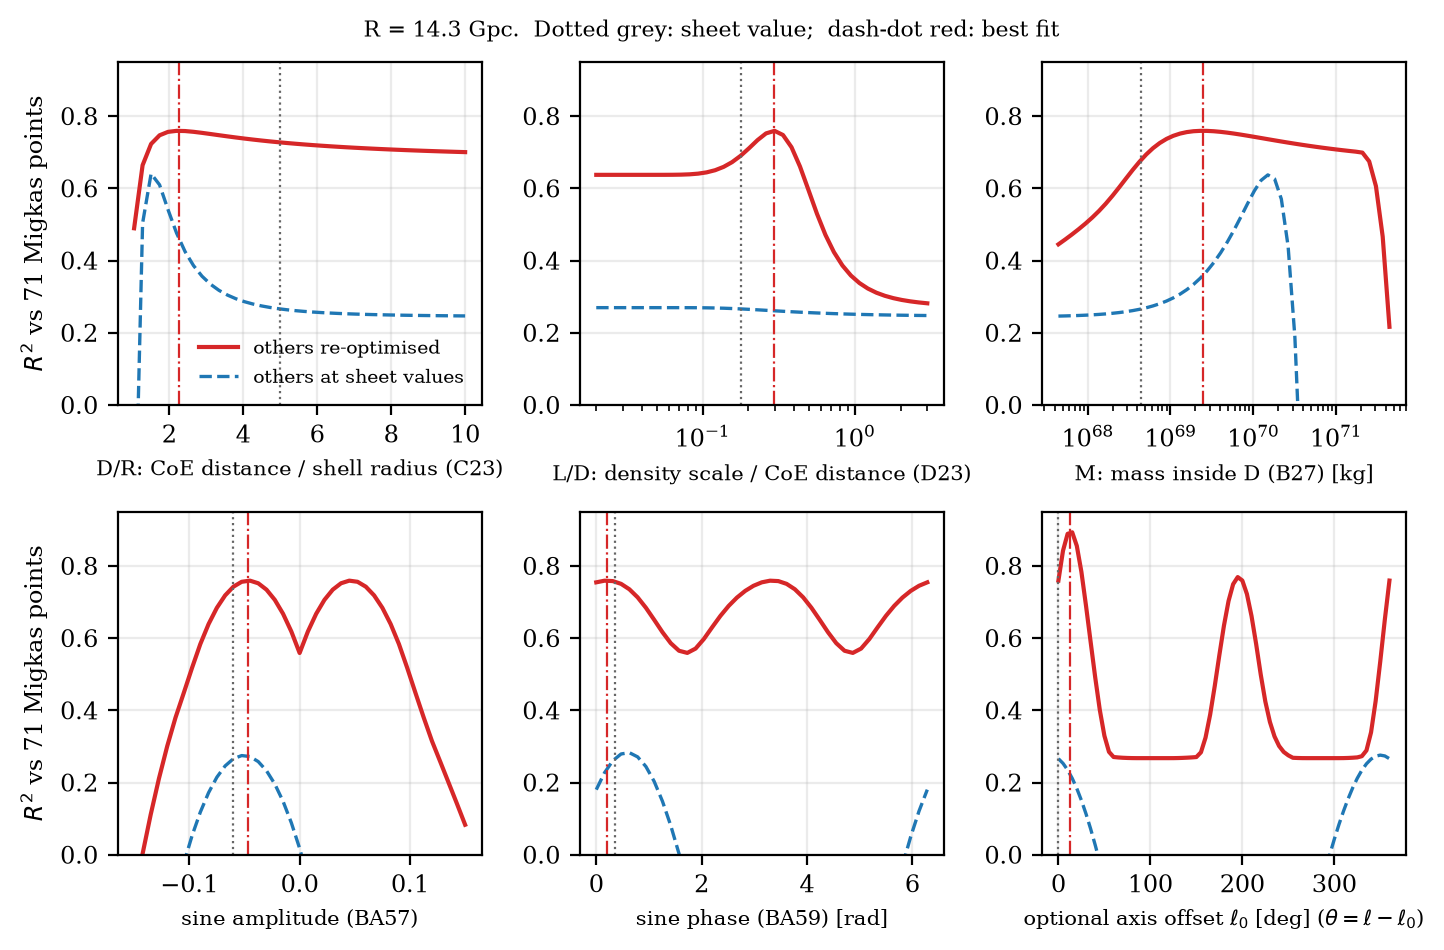
\includegraphics[width=0.84\linewidth]{param_scan_profiles.png}
\caption{$R^2$ profiles. Solid: others re-optimised. Dashed: others at sheet values.}
\end{figure}

\begin{figure}[H]\centering
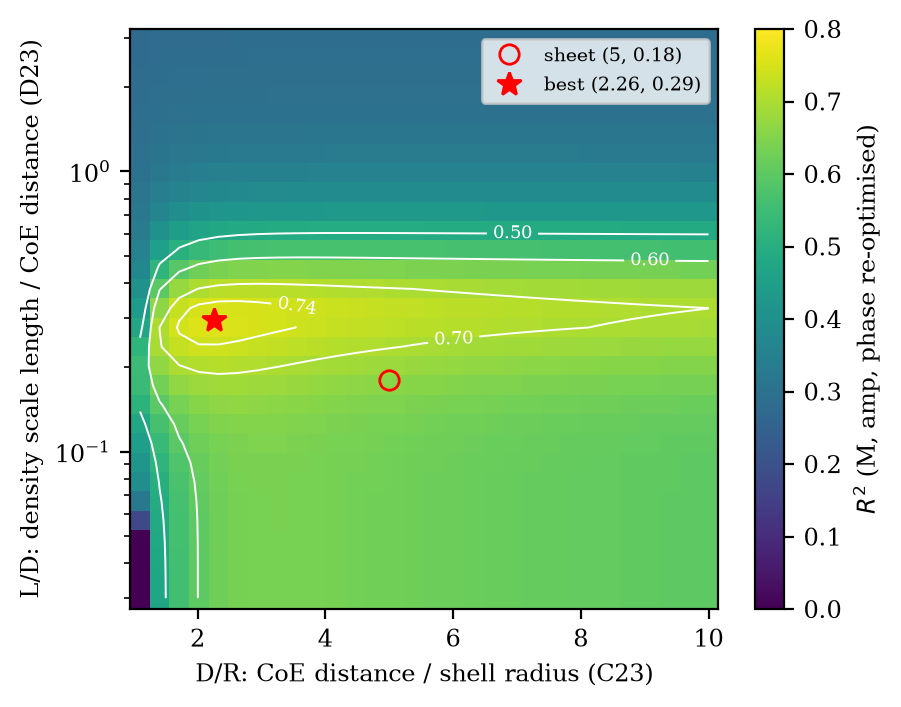
\includegraphics[width=0.48\linewidth]{param_scan_DR_LD.png}
\caption{$R^2$ over $D/R$ and $L/D$, with $M$, Amp and $\phi$ re-optimised ($\theta=\ell$).}
\end{figure}

\begin{figure}[H]\centering
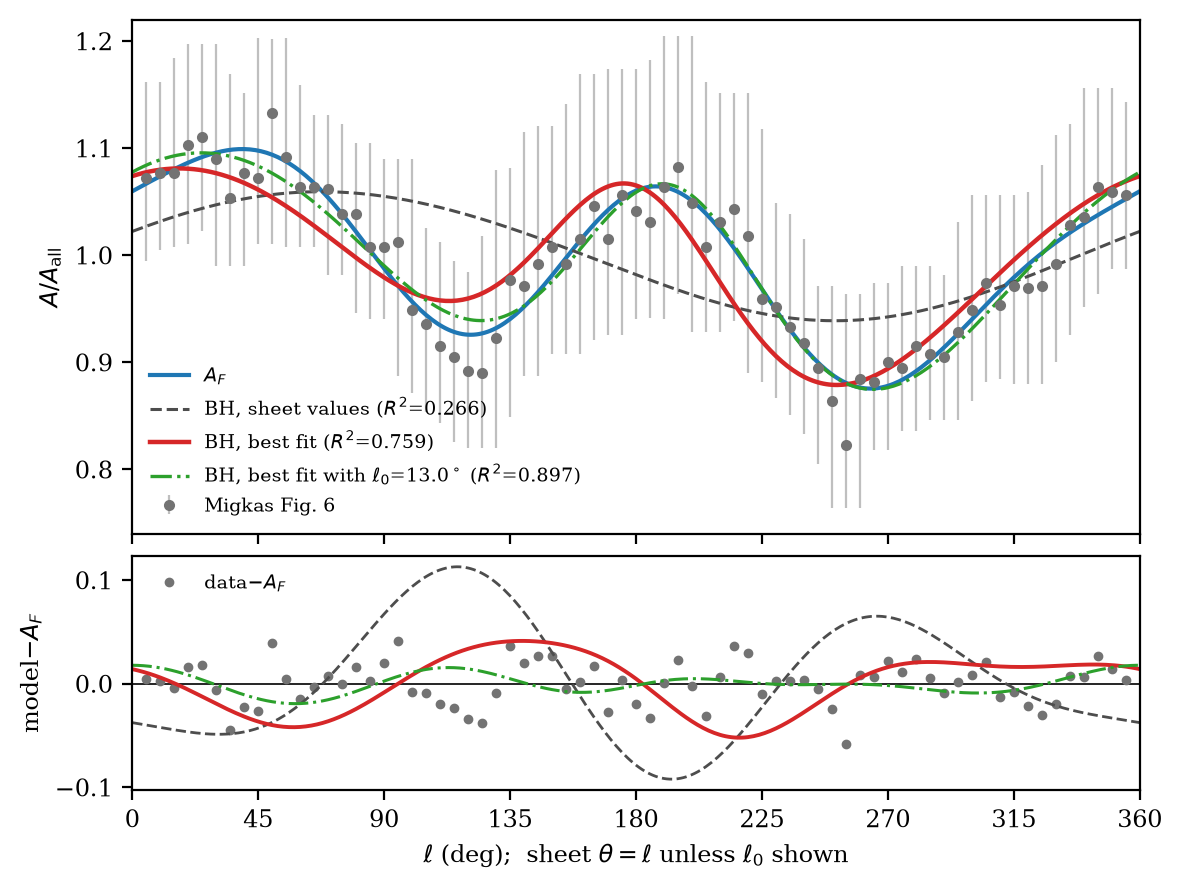
\includegraphics[width=0.7\linewidth]{param_scan_bestfit.png}
\caption{BH at the sheet values ($R=14.3$ Gpc), at the best fit, and at the best fit with $\ell_0$, compared with $A_F$ and the Migkas points.}
\end{figure}

\section{Notes}
\begin{enumerate}\setlength{\itemsep}{1pt}
\item With the bound at $1000\,M_{\rm sheet}$, no best fit or profile point is limited by $M$. The largest $M$ reached on any profile is $2.1\times10^{71}$ kg; with the old $10\times$ bound, the $D/R$ profile would have hit it.
\item The $D/R$--$M$ degeneracy remains: along the $D/R$ profile the best $M$ grows roughly as $(D/R)^3$, and $R^2$ falls only to 0.70 at $D/R=10$. $L/D=0.26$--$0.30$ is the best-determined parameter.
\item The fitted $M$ is $\sim10^{13}$--$10^{14}\,M_{\rm crit}$. This follows from $dt=1$\,s in the sheet: $\Gamma\approx0.17$ needs $GM/D^2\approx0.17\,kR$ per second. If $dt$ were $1/k$, the same $\Gamma$ would correspond to $M/M_{\rm crit}=2\Gamma(k/H_0)^2/(D/R)\approx0.14$ for the best fit. This is an interpretation, not the sheet. His $G$ is also $10^3$ times the SI value in km units.
\end{enumerate}

\end{document}
